\chapter{\textit{Plasmodium falciparum}}
\label{ch:pf}

In the previous chapter, we demonstrated our \textit{de novo} mutation detection software on simulated crossings of the \textit{falciparum} malaria parasites.  We now apply our work to real data: over $100$ samples taken from four separate crossings of six parasites.

No comprehensive catalog of \textit{de novo} variation in these crosses currently exists.  To date, the focus on the $3D7xHB3$, $HB3xDD2$, $7G8xGB4$ and $803xGB4$ datasets has largely been on discovering the genomic basis for phenotypic differences between the parents, and on characterizing novel antigenic forms in the children.  However, the previous phenotypic studies have verified the presence of some large structural \textit{de novo} variants - namely a handful of NAHR events involving antigenic genes.  These known events serve as useful validation data for the most difficult form of variation for our software to detect.  Furthermore, these previously observed events have occurred in low-complexity regions.  Such regions may confound DNA repair machinery and provide a substrate for the generation of \textit{de novo} variation.  These regions are outside the reach of reference-based analyses, but may be accessible with our graph-based approach.  Finally, the \textit{P. falciparum} genome is small enough to be sequenced inexpensively on current third generation sequencing platforms, enabling high-quality reconstructions of the parental genomes, and in turn, facilitating DNM discovery.  These factors make the \textit{P. falciparum} datasets a compelling study target.

\section{Data processing}

\subsection{Initial data}
We obtained whole genome sequence data for parent and progeny clones of the $3D7xHB3$\cite{Walliker:1987cv}, $HB3xDD2$\cite{Wellems:1990eg}, $7G8xGB4$\cite{Hayton:2008hn}, and $803xGB4$\footnote{Rick Fairhurst and Michael Krause, personal communication} crosses.  All were sequenced on Illumina platforms over the past five years using a PCR-free library preparation protocol known to reduce coverage biases associated with AT-rich templates.  Across all four crosses, we obtained $152$ samples prior to any quality control checks.

\subsection{Sample processing}

\subsubsection{Children}

We used the available Illumina data to construct the de Bruijn graph structures for each child with McCortex, using a kmer size of $47$ bp and discarding bases with a quality score less than $Q5$.  The "dirty" graph (raw graph structure before any pruning is applied) was cleaned using McCortex's automatically chosen thresholds (falling back to trimming contiguous regions of the graph with coverage less than $2$ in the event that automatic thresholds could not be calculated).  As contigs were not required for our analyses, we opted to forego the paired-end read threading and contig emission steps.

\subsubsection{Parents}
\begin{table}[]
\centering
\caption{Additional data availability for all \textit{P. falciparum} cross parents}
\label{tbl:reflist}
\begin{tabular}{@{}lllllll@{}}
\toprule
                   & 3D7 & HB3 & DD2 & 7G8 & GB4 & 803 \\ \midrule
Finished reference & x   &     &     &     &     &     \\
PacBio assembly    & x   & x   & x   & x   & x   &     \\
Draft assembly     &     & x   & x   & x   &     &     \\
Illumina data      & x   & x   & x   & x   & x   & x   \\ \bottomrule
\end{tabular}
\end{table}

In addition to the Illumina data for the parents, we often benefitted from the availability of supplementary draft assembly data from the Pf3k project.  These draft assemblies were constructed using the HGAP $2.0$ pipeline\cite{Chin:2013iw}, an assembler that follows the overlap-layout-consensus paradigm using exccedingly long reads from from PacBio RSII instruments (on average $10,000$ kb in length, sometimes as long as $50,000$ kb, two orders of magnitude longer than the reads used to assemble the finished 3D7 reference).  This data helps in determining parental paths in the graph near variants without ambiguity.  Table \ref{tbl:reflist} shows all additional data used in constructing parental assemblies.

Parental graph construction was performed on each parental data source separately following the same workflow used for the children's graphs.  The separate graphs were then combined into a single graph using McCortex's \texttt{join} command.

For most samples, the finished or draft PacBio assemblies vastly outperform any assembly that could be produced with the Illumina data, and are an excellent basis for localizing events and determining their proximity to genes.  However, as there is no high-quality sequence of the $803$ genome, we were forced to construct one ourselves using the available Illumina data.  After producing the cleaned graph with the McCortex workflow, we applied the software's paired-end read threading and contig emission steps.  The assembly statistics for all six genomes are presented in Table \ref{tbl:refstats}.  The assembly for $803$ is exceedingly poor compared to the other assemblies, as expected from short Illumina reads.  That the total sequence length is more than $2.5$ times larger than a typical \textit{falciparum} parasite is almost certainly artifactual and will be discussed further below.

\begin{table}[]
\centering
\caption{Statistics on all parental assemblies}
\label{tbl:refstats}
\begin{tabular}{@{}lllllll@{}}
\toprule
    & contigs & min length & max length & N50       & total sequence & genes            \\ \midrule
3D7 & 16      & 5,967      & 3,291,936  & 1,687,656 & 23,332,831     & 5,777            \\
DD2 & 16      & 6,094      & 3,257,617  & 1,661,885 & 22,682,339     & 8,284 (3D7, DD2) \\
7G8 & 17      & 6,094      & 3,311,228  & 1,560,458 & 22,832,195     & 5,530 (3D7)      \\
GB4 & 26      & 7,376      & 3,360,747  & 1,565,171 & 23,525,386     & 5,576 (3D7)      \\
HB3 & 28      & 6,094      & 3,378,065  & 1,593,993 & 22,812,563     & 7,467 (3D7, HB3) \\
803 & 148,826 & 47         & 17,610     & 1,042     & 59,118,463     & 4,663 (3D7)      \\ \bottomrule
\end{tabular}
\end{table}

We transferred gene models onto the new genomes by examining existing finished and draft reference genomes and their annotation sets, selecting each annotated exon sequnce from its corresponding FASTA sequence file, and aligning it to the new genome using BWA.  For 7G8, GB4, and 803, we transferred only the 3D7 annotations obtained from PlasmoDB release $26$\cite{Aurrecoechea:2009hh}.  For DD2 and HB3, additional separate annotations exist from the Broad Institute.  These undoubtedly contain better representations of genes divergent from their 3D7 counterparts (particularly antigens).  However, owing to the poor DD2 and HB3 assemblies to which they are associated, the annotations are likely to be incomplete.  We therefore chose to transfer both the 3D7 and DD2 (HB3) annotations onto the new DD2 (HB3) assemblies.  This has resulted in a slight over-annotation of genes in these two genomes, as shown in Table \ref{tbl:refstats}.  This happens when the gene models slightly differ between 3D7 and the target (e.g. exon end definitions differ by as much as a single nucleotide), but refer to the same gene.  Rather than simply choosing one definition, we permit both to remain as the PlasmoDB annotations are continuously maintained and improved, while the Broad's annotations have not been updated since April $2014$.

When producing visualizations with the Circos\cite{Krzywinski:2009ix} genomic comparison tool, we require alignments between the contigs of a parental genome and the chromosomes of the reference.  For 3D7, DD2, 7G8, GB4, and HB3, this is trivial as nearly the entirety of each chromosome has been successfully reconstructed.  For those genomes, we simply lined each assembled contig with its 3D7 counterpart.  In the case of 803, we aligned each contig to the 3D7 genome using BWA to derive the mapping.  

Finally, we computed a number of sequence composition and complexity metrics in tiled $2,500$ bp windows using the SeqComplex tool\footnote{https://github.com/caballero/SeqComplex}.  The full list of metrics computed is as follows:

\begin{enumerate}
\item gc: GC content
\item gcs: GC skew (defined as $(G - C)/(G + C)$)
\item at: AT content
\item ats: AT skew (defined as $(A - T)/(A + T)$)
\item cpg: CpG content
\item ce: Complexity by Shannon entropy\cite{Shannon:1948iy}
\item cl: Complexity by linguistic values\cite{Trifonov:1990vu}
\item cwf: Complexity by Wootton and Federhen\cite{Wootton:1996tu}
\item cz: Compression factor (the ratio of uncompressed to compressed sequence file size, using the \texttt{gzip} compression utility)
\end{enumerate}

These metrics were computed for each parental genome except 803, whose contig lengths were too variable to consistently satisfy the $2,500$ bp window requirement, making comparison with GB4 cumbersome.

\subsection{Quality control}
We examined assembly metrics on all of our samples in order to flag samples for downstream analysis rejection.  We examined each sample for outlier behavior per cross in the following metrics:

\begin{enumerate}
\item number of unique kmers: the total number of unique kmers in the graph after the automatic cleaning step
\item contig N50: the weighted median length of the contigs (very short contigs may indicate high sequencing error rate)
\item total assembly length: the sum of all contigs produced (this should be reasonably close to the expected genome size)
\end{enumerate}

The distributions for each of these metrics are shown in Figure \ref{fig:boxplotmetrics}.  We rejected samples that were outliers in at least two metrics (shown in red).

\begin{figure}[h!]
  \centering
    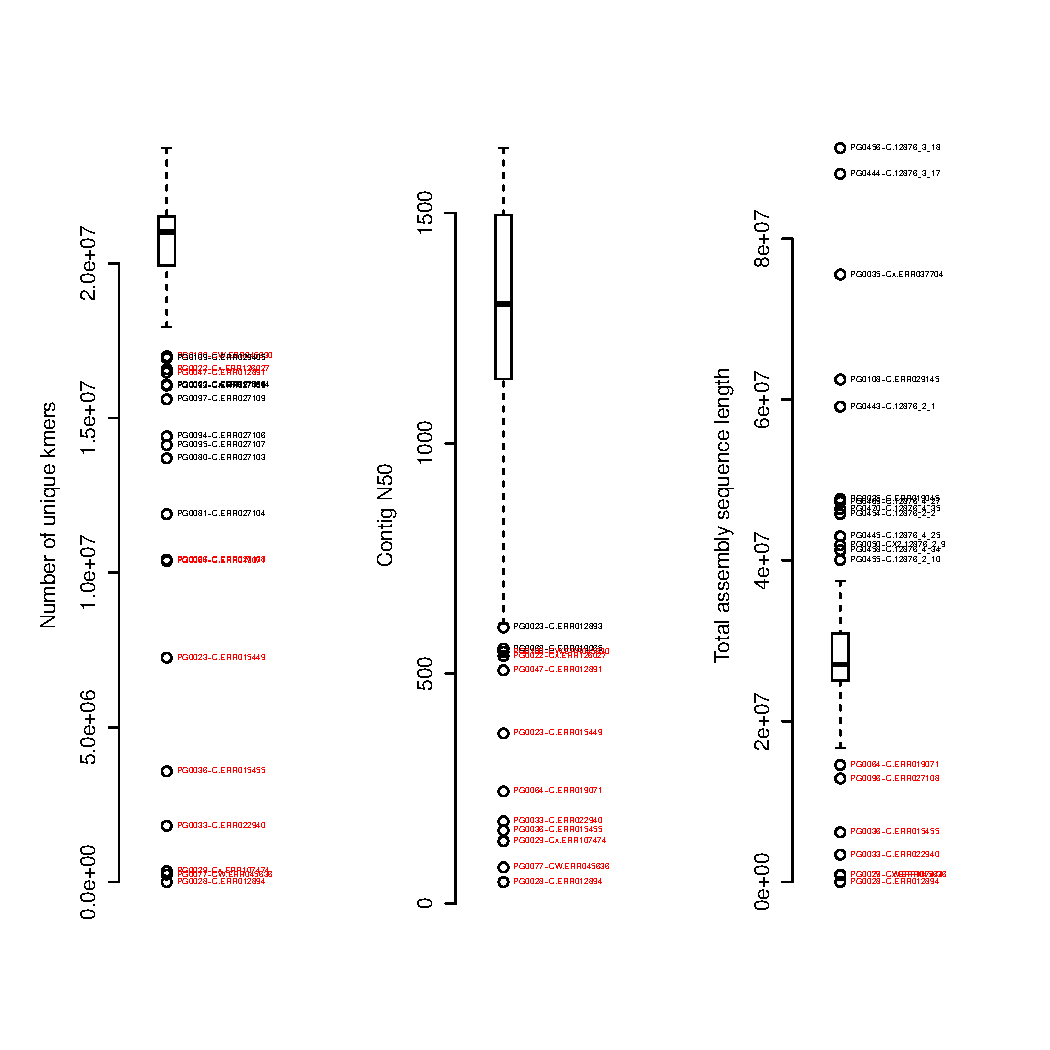
\includegraphics[width=\textwidth]{showOutliers-1}
  \caption{Boxplots of QC metrics}
  \label{fig:boxplotmetrics}
\end{figure}

One assumes that a newly assembled \textit{falciparum} parasite should have a similar assembly length to the $3D7$ reference sequence, or at least the other assembled parasites in this dataset.  Many of the $803xGB4$ samples appear to defy this expectation (including the $803$ parental sample), exhibiting assembly lengths well above the $23$ megabases we expected.  Several samples have much longer assemblies: $40$ megabases or more.  This outcome is unchanged even when other assembly software (e.g. SGA) is applied.  The source of this excess sequence is unclear.  It is possibly due to intraspecies sample contamination.  This would not be filtered out by our contamination checks, as those checks serve only to eliminate non-\textit{falciparum} kmers that might masquerade as novel kmers.  Despite this worry, we chose specifically not to exclude these samples from our analysis for two reasons: first, the issue affects a preponderance of 803xGB4 samples, including the parents; and second, our graph-based variant caller should hopefully be able to compensate for the issue.

The final dataset after QC is shown in Table \ref{tbl:crosssummary}.  Sequencing date and QC status are shown in Figure \ref{fig:gantt}.

\begin{table}[]
\centering
\caption{Summary of \textit{P. falciparum} cross data}
\label{tbl:crosssummary}
\begin{tabular}{@{}lllll@{}}
\toprule
                & 3D7xHB3       & HB3xDD2       & 7G8xGB4       & 803xGB4             \\ \midrule
Samples         & $22$          & $42$          & $52$          & $36$                \\
Samples QC+     & $21$          & $35$          & $49$          & $36$                \\
Read length     & $76$          & $76$          & $76$          & $100$               \\
Fragment size   & $300 \pm 29$  & $253 \pm 48$  & $293 \pm 21$  & $222 \pm 10$        \\
Coverage        & $99  \pm 38$  & $121 \pm 91$  & $110 \pm 40$  & $205 \pm 106$       \\
Platform        & Illumina GAII & Illumina GAII & Illumina GAII & Illumina HiSeq 2000 \\
Sequencing Date & 2010          & 2009-2012     & 2010-2011     & 2014                \\ \bottomrule
\end{tabular}
\end{table}

\begin{landscape}
  \begin{figure}[h!]
    \centering
      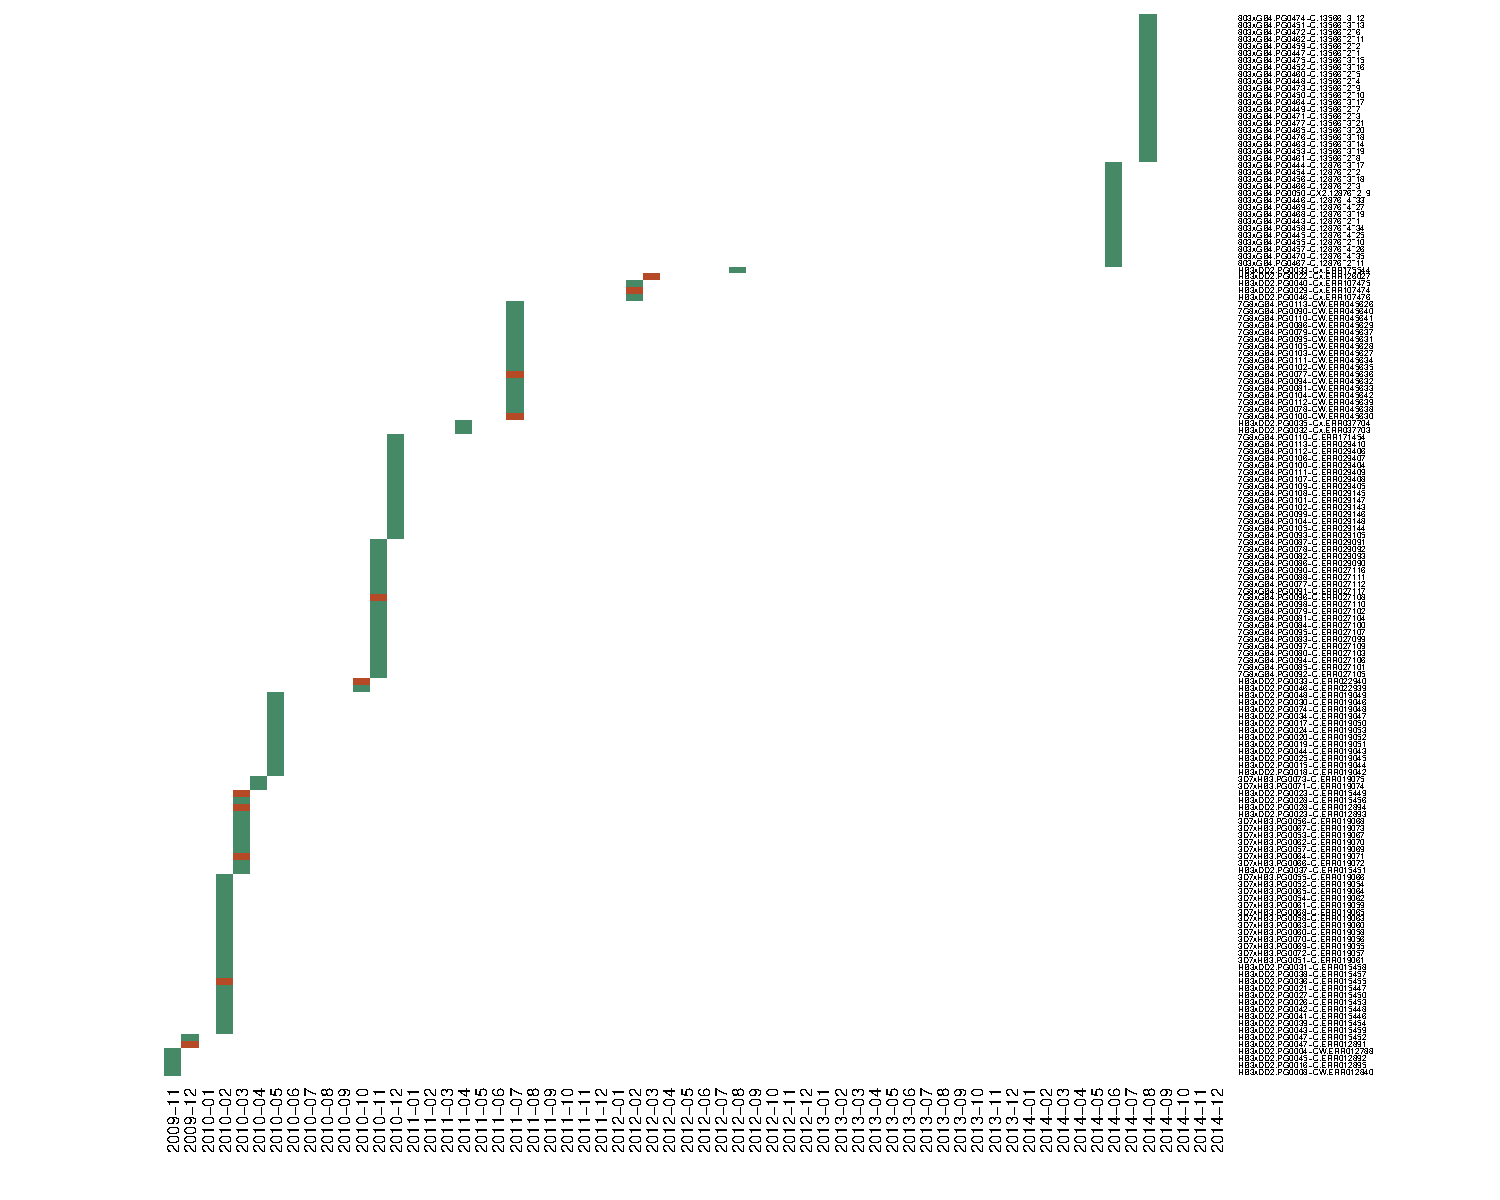
\includegraphics[width=\textwidth]{gantt-1}
    \caption{Samples and their sequencing date.  QC failures are shown in red.}
    \label{fig:gantt}
  \end{figure}
\end{landscape}

\subsection{Novel kmers}

We identified novel kmers using the software we presented in Chapter \ref{ch:methods}, dividing the set into three subsets: "all" (no filtering applied), "confident" (kmer coverage thresholds automatically detected and applied), and "trusted" (potential contaminants removed).  The total number of such kmers is shown in Figure \ref{fig:novelty}a.

The 3D7xHB3 cross has far more novel kmers than the other samples before any coverage and contamination filters are applied.  This may simply reflect the fact that the 3D7xHB3 samples were sequenced on early Illumina GAII sequencers and chemistry.  With the exception of a handful of HB3xDD2 samples, they are the oldest samples in the dataset, and perhaps have a much higher error rate to show for it.

Furthermore, the 803xGB4 samples have consistent novel kmer behavior with the samples from other crosses, despite the assembly lengths being substantially longer than expectation.

\begin{figure}
\begin{subfigure}{.5\textwidth}
  \centering
  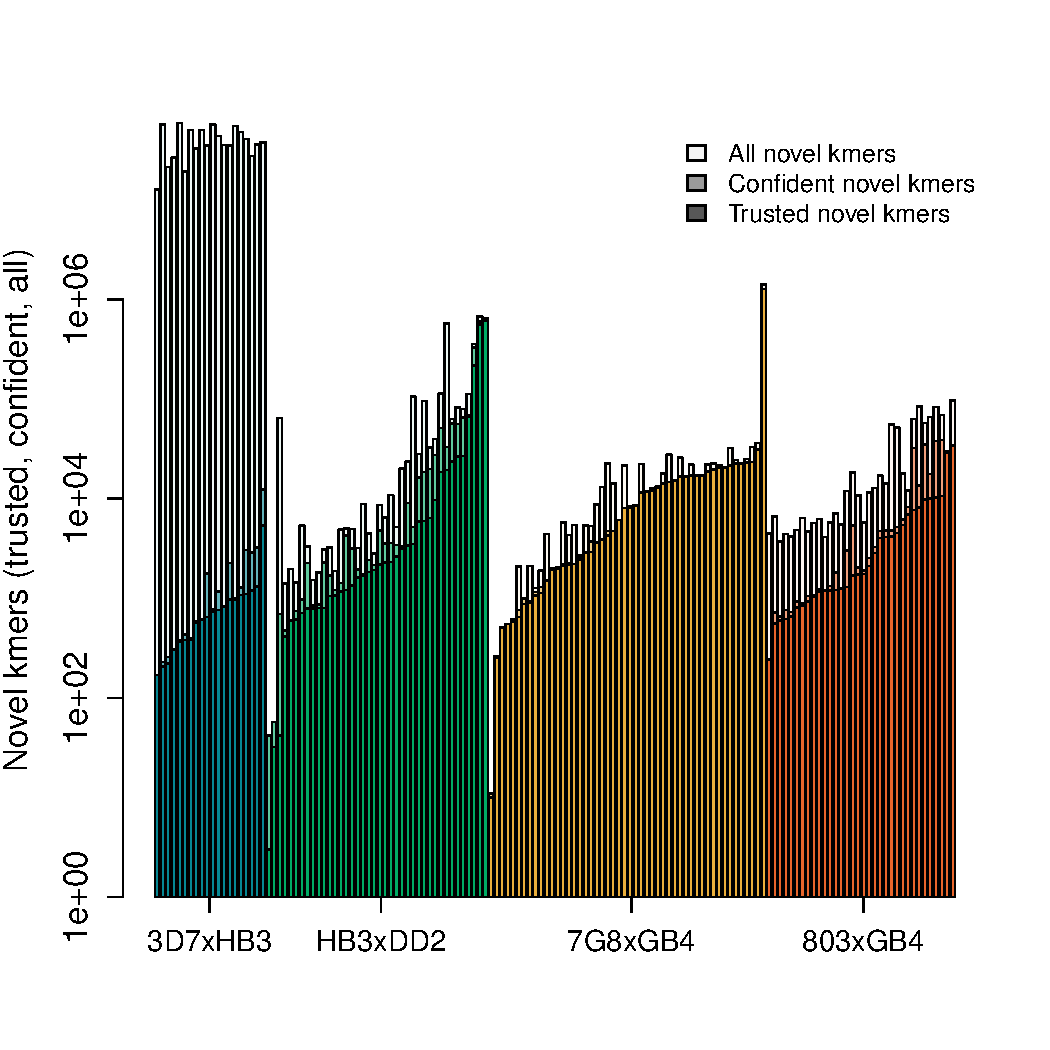
\includegraphics[width=\linewidth]{novelKmers-1}
  %\caption{Confident and trusted novel kmers per sample}
  \label{fig:novelKmers-1}
\end{subfigure}%
\begin{subfigure}{.5\textwidth}
  \centering
  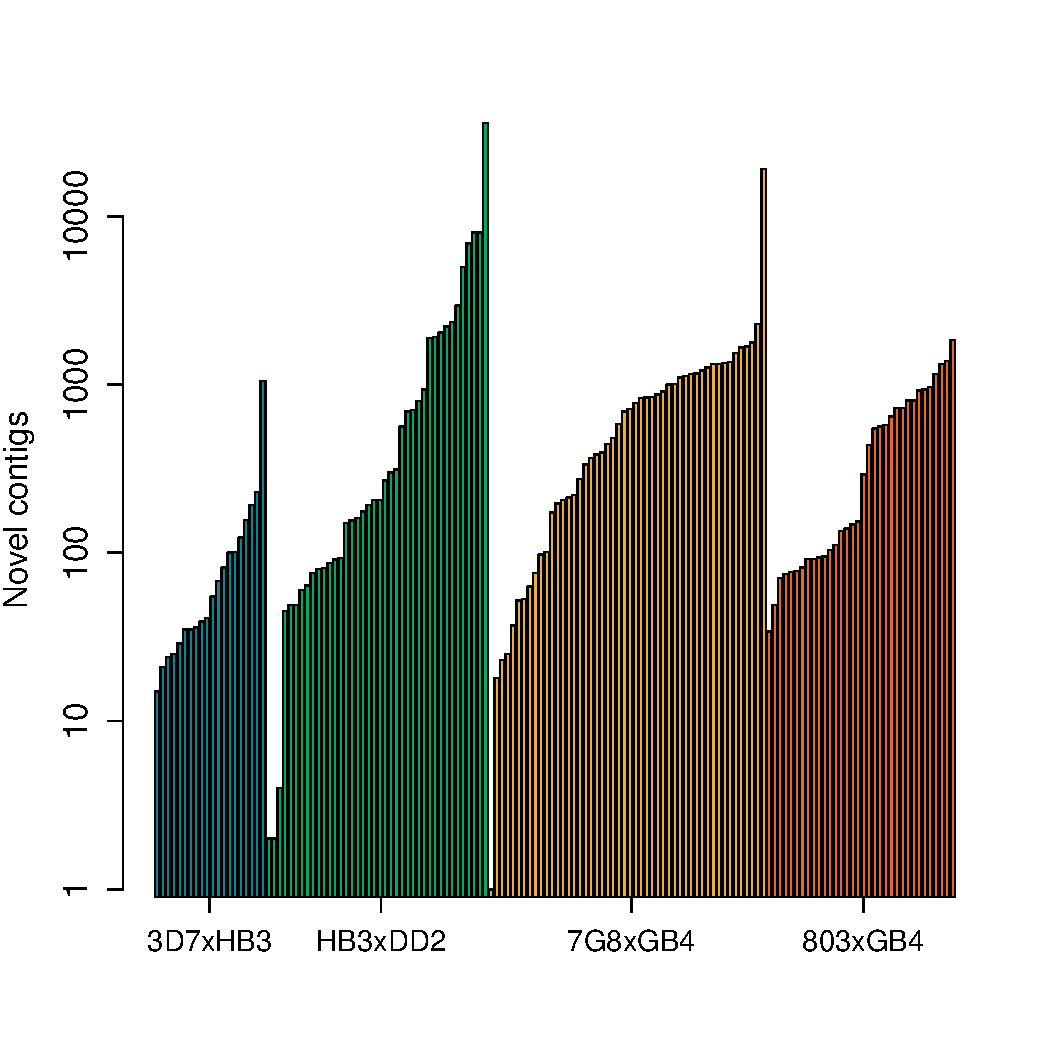
\includegraphics[width=\linewidth]{novelStretches-1}
  %\caption{Ns vs nk}
  \label{fig:novelStretches-1}
\end{subfigure}
\caption{a. Number of novel kmers found in each sample, broken down into "trusted", "confident", and "all" categories.  b. Number of novel contigs (contigs containing at least one trusted novel kmer) per sample.}
\label{fig:novelty}
\end{figure}

After all filters are applied, the number of novel kmers per sample appears to have tremendous variance, typically between $100$ and $1,000$.

Novel contigs (contigs containing trusted novel kmers) can be used as a proxy for \textit{de novo} mutations in the genome, as each contiguous stretch of novel kmers ideally represents the child's branch of a variant bubble.  In practice, the proxy is imperfect as many contigs will be prematurely truncated due to absent coverage, repetitive regions, or sequencing error.  Nevertheless, it is still a useful upper bound on the amount of variation we might expect to see in each parasite.  Figure \ref{fig:novelty}b shows the number of such novel contigs in each sample.  The median number of novel contigs per sample is $224$, far fewer in the 3D7xHB3 cross ($48$).  The overall contig count distributions are quite consistent between crosses.

\section{\textit{De novo} mutations in the \textit{P. falciparum} crosses}

\subsection{\textit{De novo} mutations in a single sample}

We first examined DNM calls in a single sample from the $3D7xHB3$ cross: PG0063-C.  This sample is known to harbor an NAHR event between two \textit{var} genes: $PF3D7\_0100100$ (situated in the 5' telomere of chromosome $1$), and $PF3D7\_0223500$ (the 3' telomere of chromosome $2$), which makes it a useful test sample for initial examination.  All $27$ called mutations are described in Table \ref{tbl:callsPG0063C}, additionally annotated with the locus, the haplotypic background of the variant, variant type, closest gene (and the associated product), and whether the variant falls within the MalariaGen variant calling exclusion mask.  The variants can be seen in their genomic context in Figure \ref{fig:circosPG0063C}.  

\begin{landscape}
\begin{table}[]
\centering
\caption{\textit{De novo} variants in 3D7xHB3 progeny, PG0063-C}
\label{tbl:callsPG0063C}
\begin{tabular}{@{}lllllll@{}}
\toprule
   & locus               & background &  event    &  closest gene                   &  product          &  within mask  \\
\midrule
1      & 1:27733             & 3D7        &  unknown  &  PF3D7\_0100100                 &  PfEMP1 (var)     &  yes          \\
2      & 1:29780             & 3D7        &  MNP      &  PF3D7\_0100100                 &  PfEMP1 (var)     &  yes          \\
3      & 1:30339;2:922666    & 3D7        &  NAHR     &  PF3D7\_0100100;PF3D7\_0223500* &  PfEMP1 (var)     &  yes          \\
4      & 1:31825;2:920323    & 3D7        &  unknown  &  PF3D7\_0100100;PF3D7\_0223500* &  PfEMP1 (var)     &  yes          \\
5      & 1:30503;1:613915    & 3D7        &  NAHR     &  PF3D7\_0115700                 &  PfEMP1 (var)     &  yes          \\
6      & 2:227               & 3D7        &  NAHR     &  PF3D7\_0200100                 &  PfEMP1 (var)     &  yes          \\
7      & 2:394194            & 3D7        &  unknown  &  PF3D7\_0209600*                &  transporter      &  no           \\
8      & 2:919803            & 3D7        &  SNP      &  PF3D7\_0223500*                &  PfEMP1 (var)     &  yes          \\
9      & 3:471               & HB3        &  unknown  &  PF3D7\_0300100                 &  PfEMP1 (var)     &  yes          \\
10     & 3:1064983           & 3D7        &  unknown  &  PF3D7\_0324900                 &  PfEMP1 (var)     &  yes          \\
11     & 6:1338957           & HB3        &  GC       &  PF3D7\_0632100*                &  RIF              &  yes          \\
12     & 6:1338975           & HB3        &  unknown  &  PF3D7\_0632100*                &  RIF              &  yes          \\
13     & 7:658               & HB3        &  MNP      &  PF3D7\_0700100                 &  PfEMP1 (var)     &  yes          \\
14     & 7:1428132           & 3D7        &  INS      &  PF3D7\_0733000                 &  PfEMP1 (var)     &  yes          \\
15     & 10:1663367          & 3D7        &  MNP      &  PF3D7\_1041300                 &  PfEMP1 (var)     &  yes          \\
16     & 12:532              & 3D7        &  unknown  &  PF3D7\_1200100                 &  PfEMP1 (var)     &  yes          \\
17     & 12:603510;12:603561 & 3D7        &  unknown  &  PF3D7\_1214100*                &  PIGO             &  no           \\
18     & 13:953155           & HB3        &  unknown  &  PF3D7\_1322500*                &  DHHC5            &  no           \\
19     & 13:15776184         & HB3        &  unknown  &  PF3D7\_1339200                 &  tRNA proline     &  no           \\
20     & 13:2871396          & 3D7        &  STR\_EXP &  PF3D7\_1373100*                &  RIF              &  yes          \\
21     & 14:1040207          & 3D7        &  unknown  &  PF3D7\_1426700                 &  PEPC             &  no           \\
22     & 14:3016814          & 3D7        &  SNP      &  PF3D7\_1474000*                &  probable protein &  no           \\
23     & 14:3065820          & 3D7        &  unknown  &  PF3D7\_1474700*                &  protein kinase   &  no           \\
24 (a) & 1:27241;14:23321    & 3D7;HB3    &  NAHR     &  PF3D7\_0100100;PF3D7\_1400700  &  Stevor;PfEMP1 (var) & yes        \\
24 (b) & 14:23321;1:617342   & HB3;3D7    &  NAHR     &  PF3D7\_1400700;PF3D7\_0115700  &  PfEMP1 (var)     &  yes          \\
24 (c) & 1:617342;13:2894565 & 3D7        &  NAHR     &  PF3D7\_0115700;PF3D7\_1373500  &  PfEMP1 (var)     &  yes          \\
25     & NA                  & 3D7        &  unknown  &  unknown                        &  unknown          &  NA           \\
26     & NA                  & 3D7        &  unknown  &  unknown                        &  unknown          &  NA           \\
27     & NA                  & 3D7        &  unknown  &  unknown                        &  unknown          &  NA           \\
\bottomrule
\end{tabular}
\end{table}
\end{landscape}

\begin{figure}[h!]
  \centering
    \includegraphics[width=\textwidth]{{PG0063-C.ERR019060.circos}.png}
  \caption{Circos visualization of all \textit{de novo} mutations in PG0063-C, positioned on the reference sequence (outer ring), aligned maternal assembly (middle), and aligned paternal assembly (inner).  Unplaced parental contigs are concatenated and placed in the "U" pseudochromosome.  Each parental ring is annotated with a sequence compressibility score for every $2,500$ bp shown above their ideograms, while the reference ring is annotated with mean read coverage per $2,500$ bp.  Within the reference ideogram, all reference-based variant calls made in this sample from the MalariaGen project are shown, color-coded to reflect their parentage.  Regions that were masked out of MalariaGen's variant calling process are shown as grey bars.  Variants are shown as glyphs below the parental ideograms, shape-coded for type (small circle: unknown, large circle: SNP, triangle: indel, square: MNP, diamond: NAHR event).  The color and positioning of the glyph reflects the haplotypic background upon which the event occurred.  Interchromosomal structural variation and gene-conversion events are additionally denoted as arcs linking the relevant parts of the genome.  The closest gene to the event is reported in black if the mutation falls within the gene and as grey if it falls outside the gene.}
  \label{fig:circosPG0063C}
\end{figure}

There are several noteworthy features of Table \ref{tbl:callsPG0063C} and Figure \ref{fig:circosPG0063C}.  First, the call rate is reasonably low; less than $30$ events in this sample, consistent with the expectation that \textit{de novo} mutations should be rare.  We discover a variety of event types, including SNPs (depicted in the plot with large circles), indels (triangles), multi-nucleotide polymorphisms (squares), and NAHR events (diamonds).  Many events could not be typed (small circles).

Second, nearly all of the events can be localized within the parental genomes, even if the precise event type could not always be determined.  Here, we benefit from aligning sequences that flank the region of novelty, rather than aligning $76$ bp reads.  The flanking sequences can often be longer than a read length, which provides the alignment software more context with which to determine an appropriate home for the variant.  Further to this point, nearly all of the variants appear on a haplotypic background consistent with the haplotype assignments from the reference-based analysis (shown in the outer ideogram).  This is of course expected, as when the graph traversal lacks sufficent context to determine the parentage of a stretch of sequence, we simply determine the appropriate parent using the flank alignments and the reference-based parentage determinations.  There are occasional violations of the expected parentage, which may indicate a missed recombination event (perhaps a gene conversion in the case of the untyped variant at the 3' end of chromosome $3$).

Third, we are able to identify interchromosomal exchanges, including the known NAHR event between PF3D7\_0100100 on the 5' end of chromosome $1$ and PF3D7\_0223500 on the 3' end of chromosome $2$\cite{Anonymous:2013hi}.  Curiously, there is another apparent interchromosomal exchange involving antigenic genes on chromosomes $1$, $13$, and $14$.  While Sander \textit{et al.} did describe another NAHR event involving PF3D7\_0115700 and PF3D7\_0200100, that event was verified to have occurred in PG0062-C, not PG0063-C.  Both PF3D7\_0115700 and PF3D7\_0200100 do seem to have incurred DNMs.  However, our calls suggest an exchange between PF3D7\_0115700, PF3D7\_1373500 (both \textit{var} genes), and perhaps even PF3D7\_1400700 (a member of the \textit{stevor} antigenic gene family).  Such a complex recombination seems implausible, and is perhaps artifactual.  This unexpected behavior might be due to intraspecies contamination during library preparation of the sequenced samples.  However, if significant sample mixing had occurred, we would expect to see unusual allele balances at variant sites in the reference-based analysis (since in a pure sample, the allele balance should ideally be $100\%$ alternate allele, $0\%$ reference allele).  Visual inspection of a number of variant sites in IGV does not reveal unusual allele balances.  We note that the alignment of this variant's flanking sequence to chromosomes $13$ and $14$ are only supported by $2$ to $4$ kmers ($48$ to $50$ bp, respectively).  It is possible that a repetitive region present on all three chromosomes happens to be collapsed on chromosome $1$, but represented more completely on chromosomes $13$ and $14$.  Kmers that appear unique to those chromosomes might actually be present in chromosome $1$, but are not present in the finished sequence by chance.

Fourth, we are able to detect some intrachromosomal events.  Chromosome $6$ appears to contain a single gene conversion event within the PF3D7\_0632100 gene, a member of the large \textit{rifin} antigenic gene family.  Interestingly, chromosome $2$ is home to a variant whose type was unable to be determined.  However, it is apparently on the 3D7 haplotypic background, despite surrounding variants suggesting that it should be on the HB3 background.  This could be another gene conversion event that was incompletely assembled.

Fifth, we are able to detect many mutations that occur in masked regions of the reference genome.  MalariaGen delibrately excluded a number of regions from processing.  This included repetitive regions (often telomeric, centromeric, or pericentromeric regions) as short reads could often not be aligned in long repetitive regions with confidence.  It also included hypervariable regions (typically subtelomeric) as population diversity was too great to yield confident results in the reference-based analysis.  As we are comparing each sample to a parental graph rather than a reference sequence that is an undetermined number of generations removed, our graphical approach can reconstruct and localize these events.  For example, the MNP on the 3' end of chromosome $10$ falls within a subtelomeric repetitive region.

Sixth, our calls in this sample appear overwhelmingly concentrated in or near antigenic genes ($19$/$27$), most often \textit{var} genes.  This is likely somewhat over-counted owing to incomplete reconstructions of the same variant appearing multiple times.  Yet, a more pessimistic accounting wherein we only count each affected locus once still suggests that $14$/$23$ events are in or near antigenic genes.  Such a skew is unusual, especially given the fact that our algorithm is hypothesis-free and is not biased towards processing any particular region of the genome.

Subtelomeric regions (and the antigenic genes contained within) are known to be high in repetitive sequence.  To visualize the potential relationship between sequence content and variant location, we examined a number of different sequence properties.  Shown in Figure \ref{fig:circosPG0063C} above each parental assembly track is one of these metrics: the sequence compression ratio.  Data compression algorithms look for a smaller representation of a given string of data.  For example, a simple run-length encoding (wherein we count the number of identical and adjacent characters) of the sequence \texttt{AAAAGAGACCCC} might yield the encoding,

\begin{equation}
rle(AAAAGAGACCCC) = A(4)G(1)A(1)G(1)A(1)C(4) ,
\end{equation}

\noindent where the number indicates the the preceeding character should be repeated in order to reconstruct the original sequence.  In contrast, the sequence \texttt{AGTCGTTCATGT} would yield,

\begin{equation}
rle(AGTCGTTCATGT) = A(1)G(1)T(1)C(1)G(1)T(2)C(1)A(1)T(1)G(1)T(1) .
\end{equation}

\noindent Clearly the first sequence compresses to something much smaller than the second owing to the repetitiveness of the sequence.  Such compression or entropy measures on sequence provide an excellent metric for sequence complexity.  Many of our DNM calls appear to follow closely with spikes in the local sequence compressibility measure.  Quite often these spikes correspond with being in a masked repetitive region, but there are notable additions.  For example, two SNPs on chromosome $14$, occuring in PF3D7\_1474000 (unknown function) and PF3D7\_1474700 (a protein kinase, thought to be a viable drug target\cite{Talevich:2011ei}) appear near such a local increase in sequence compressibility.  We shall examine this point in greater detail when we discuss the calls across the whole dataset.

\subsection{\textit{De novo} mutations in all 3D7xHB3 progeny}

\subsubsection{Allelic events}

\begin{figure}[h!]
  \centering
    \includegraphics[width=\textwidth]{{variantTypes-1}.pdf}
  \label{fig:3D7xHB3variantTypes}
  \caption{\textit{De novo} mutations in each of the $20$ progeny from the 3D7xHB3 cross.}
\end{figure}

Counts per sample are shown in Figure \ref{fig:3D7xHB3variantTypes}, stratified by type (left) and subtype (right).  Across the entire $20$-sample 3D7xHB3 dataset, allelic variant counts per sample are modest - around two SNPs and one to two insertions, deletions, and MNPs per sample.  Many of these events are still found in subtelomeric low complexity regions, as evidenced by the sample mosaic in Figure \ref{fig:3D7xHB3circos}.

\begin{figure}[h!]
  \centering
    \includegraphics[width=\textwidth]{{3D7xHB3.circos.first_half}.pdf}
\end{figure}

\begin{figure}[h!]
  \centering
    \includegraphics[width=\textwidth]{{3D7xHB3.circos.second_half}.pdf}
  \caption{\textit{De novo} mutations in each of the $20$ progeny from the 3D7xHB3 cross.  Left: mutations stratified by type.  Right: mutations stratified by subtype.}
  \label{fig:3D7xHB3circos}
\end{figure}

\begin{landscape}
\centering
\small
\begin{longtable}{llrlll}
\toprule
sample & type & length & locus & gene & description \\
\midrule
PG0063-C.ERR019060 & MNP & 0 & Pf3D7\_01\_v3:27733-27902 & PF3D7\_0100100 & PfEMP1 (VAR)\\
PG0063-C.ERR019060 & MNP & 9 & Pf3D7\_01\_v3:29780-30133 & PF3D7\_0100100* & PfEMP1 (VAR)\\
PG0061-C.ERR019059 & DEL & 30 & PfHB3\_01:299430-299547 & PF3D7\_0108700* & secreted ookinete protein, putative (PSOP24)\\
PG0055-C.ERR019066 & SNP & 0 & Pf3D7\_02\_v3:495067-495161 & PF3D7\_0212400 & conserved membrane protein, unknown function\\
PG0053-C.ERR019067 & SNP & 0 & Pf3D7\_02\_v3:495067-495161 & PF3D7\_0212400 & conserved membrane protein, unknown function\\
PG0070-C.ERR019056 & SNP & 0 & PfHB3\_02:698465-698559 & PF3D7\_0217500* & calcium-dependent protein kinase 1 (CDPK1)\\
PG0063-C.ERR019060 & SNP & 0 & Pf3D7\_02\_v3:919803-920297 & PF3D7\_0223500* & PfEMP1 (VAR)\\
PG0062-C.ERR019070 & INS & 100 & PfHB3\_04:1-48 & PF3D7\_0300600 & exported protein, unknown function, fragment\\
PG0062-C.ERR019070 & INS & 100 & Pf3D7\_03\_v3:1063591-1063645 & PF3D7\_0324900 & PfEMP1 (VAR)\\
PG0053-C.ERR019067 & MNP & 2 & Pf3D7\_03\_v3:1066484-1066640 & PF3D7\_0324900 & PfEMP1 (VAR)\\
PG0061-C.ERR019059 & SNP & 0 & Pf3D7\_05\_v3:31612-31706 & PF3D7\_0500400 & rifin (RIF)\\
PG0066-C.ERR019072 & DEL & 32 & Pf3D7\_05\_v3:208520-208614 & PF3D7\_0505000 & conserved membrane protein, unknown function\\
PG0055-C.ERR019066 & SNP & 0 & PfHB3\_05:1147154-1147246 & PF3D7\_0527300 & methionine aminopeptidase 1a, putative (METAP1a)\\
PG0053-C.ERR019067 & MNP & 10 & PfHB3\_05:1203344-1203449 & PF3D7\_0529100 & conserved protein, unknown function\\
PG0071-C.ERR019074 & DEL & 102 & Pf3D7\_06\_v3:57319-57486 & PF3D7\_0601400 & PfEMP1 (VAR) pseudogene\\
PG0070-C.ERR019056 & STR\_CON & 4 & Pf3D7\_06\_v3:253909-253981 & PF3D7\_0606000 & conserved protein, unknown function\\
PG0064-C.ERR019071 & MNP & 54 & Pf3D7\_06\_v3:1416554-1416719 & PF3D7\_0632800 & PfEMP1 (VAR)\\
PG0071-C.ERR019074 & STR\_EXP & 2 & Pf3D7\_06\_v3:1377300-1377366 & PF3D7\_0632800* & PfEMP1 (VAR)\\
PG0056-C.ERR019068 & SNP & 0 & PfHB3\_07:1102288-1102382 & PF3D7\_0727700* & conserved protein, unknown function\\
\addlinespace
PG0072-C.ERR019057 & MNP & 26 & Pf3D7\_07\_v3:1428612-1428810 & PF3D7\_0733000 & PfEMP1 (VAR)\\
PG0063-C.ERR019060 & INS & 1 & Pf3D7\_07\_v3:1428132-1428267 & PF3D7\_0733000 & PfEMP1 (VAR)\\
\addlinespace
PG0068-C.ERR019065 & STR\_CON & 8 & PfHB3\_08:79631-79699 & PF3D7\_0801500 & nucleolar protein 10, putative (NOL10)\\
PG0053-C.ERR019067 & MNP & 34 & PfHB3\_04:478252-478977 & PF3D7\_0809000 & RNA of unknown function RUF6-10\\
\addlinespace
PG0067-C.ERR019073 & STR\_CON & 8 & Pf3D7\_08\_v3:656614-656684 & PF3D7\_0813300 & conserved protein, unknown function\\
PG0055-C.ERR019066 & STR\_CON & 8 & Pf3D7\_08\_v3:656614-656684 & PF3D7\_0813300 & conserved protein, unknown function\\
PG0053-C.ERR019067 & STR\_CON & 8 & Pf3D7\_08\_v3:656614-656684 & PF3D7\_0813300 & conserved protein, unknown function\\
PG0056-C.ERR019068 & STR\_CON & 8 & Pf3D7\_08\_v3:656614-656684 & PF3D7\_0813300 & conserved protein, unknown function\\
\addlinespace
PG0055-C.ERR019066 & DEL & 947 & Pf3D7\_08\_v3:1024822-1025845 & PF3D7\_0823200 & RNA binding protein, putative\\
PG0068-C.ERR019065 & STR\_EXP & 5 & PfHB3\_09:217009-217114 & PF3D7\_0905100 & nucleoporin NUP100/NSP100, putative (NUP100)\\
PG0061-C.ERR019059 & DEL & 15 & Pf3D7\_09\_v3:472149-472252 & PF3D7\_0910300 & conserved protein, unknown function\\
PG0073-C.ERR019075 & STR\_CON & 8 & Pf3D7\_09\_v3:1223097-1223182 & PF3D7\_0930700* & conserved protein, unknown function\\
PG0073-C.ERR019075 & MNP & 110 & Pf3D7\_10\_v3:145-377 & PF3D7\_1000100 & PfEMP1 (VAR)\\
PG0069-C.ERR019055 & STR\_EXP & 2 & PfHB3\_10:581292-581364 & PF3D7\_1015700.1 & tubulin binding cofactor c, putative\\
PG0066-C.ERR019072 & SNP & 0 & Pf3D7\_10\_v3:1286013-1286107 & PF3D7\_1031900* & conserved protein, unknown function\\
PG0068-C.ERR019065 & SNP & 0 & PfHB3\_10:1263212-1263306 & PF3D7\_1032700 & conserved protein, unknown function\\
\addlinespace
PG0062-C.ERR019070 & SNP & 0 & PfHB3\_10:1396068-1396162 & PF3D7\_1036500 & probable protein, unknown function\\
PG0065-C.ERR019064 & SNP & 0 & PfHB3\_10:1396068-1396162 & PF3D7\_1036500 & probable protein, unknown function\\
\addlinespace
PG0063-C.ERR019060 & MNP & 147 & Pf3D7\_10\_v3:1663367-1663662 & PF3D7\_1041300 & PfEMP1 (VAR)\\
PG0056-C.ERR019068 & INS & 89 & Pf3D7\_10\_v3:1687367-1687443 & PF3D7\_1041300 & PfEMP1 (VAR)\\
\addlinespace
PG0070-C.ERR019056 & MNP & 6 & Pf3D7\_11\_v3:448-545 & PF3D7\_1100100 & PfEMP1 (VAR)\\
PG0058-C.ERR019063 & MNP & 87 & Pf3D7\_11\_v3:26051-26674 & PF3D7\_1100100* & PfEMP1 (VAR)\\
PG0071-C.ERR019074 & INS & 1 & Pf3D7\_11\_v3:66678-66762 & PF3D7\_1101100* & rifin (RIF)\\
\addlinespace
PG0062-C.ERR019070 & STR\_CON & 4 & Pf3D7\_11\_v3:82697-82754 & PF3D7\_1101600* & exported protein (hyp4), unknown function\\
PG0065-C.ERR019064 & STR\_CON & 4 & Pf3D7\_11\_v3:82697-82754 & PF3D7\_1101600* & exported protein (hyp4), unknown function\\
\addlinespace
PG0073-C.ERR019075 & SNP & 0 & Pf3D7\_11\_v3:1019513-1019607 & PF3D7\_1126100* & ThiF family protein, putative\\
PG0069-C.ERR019055 & SNP & 0 & Pf3D7\_11\_v3:1019513-1019607 & PF3D7\_1126100* & ThiF family protein, putative\\
\addlinespace
PG0073-C.ERR019075 & STR\_EXP & 5 & PfHB3\_11:1662431-1662485 & PF3D7\_1143700 & conserved protein, unknown function\\
PG0054-C.ERR019062 & STR\_EXP & 4 & Pf3D7\_11\_v3:2016514-2016581 & PF3D7\_1150100 & rifin, pseudogene (RIF)\\
PG0072-C.ERR019057 & MNP & 75 & PfHB3\_12:768277-768511 & PF3D7\_1219400 & PfEMP1 (VAR) pseudogene\\
\addlinespace
PG0067-C.ERR019073 & STR\_EXP & 2 & Pf3D7\_12\_v3:875371-875426 & PF3D7\_1222000 & conserved protein, unknown function\\
PG0055-C.ERR019066 & STR\_EXP & 2 & Pf3D7\_12\_v3:875371-875426 & PF3D7\_1222000 & conserved protein, unknown function\\
PG0053-C.ERR019067 & STR\_EXP & 2 & Pf3D7\_12\_v3:875371-875426 & PF3D7\_1222000 & conserved protein, unknown function\\
\addlinespace
PG0057-C.ERR019069 & SNP & 0 & Pf3D7\_12\_v3:2264188-2264282 & PF3D7\_1255200 & PfEMP1 (VAR)\\
PG0054-C.ERR019062 & DEL & 87 & Pf3D7\_13\_v3:412-600 & PF3D7\_1300100 & PfEMP1 (VAR)\\
PG0061-C.ERR019059 & SNP & 0 & Pf3D7\_13\_v3:773695-773789 & PF3D7\_1318800 & secretory complex protein 63 (SEC63)\\
\addlinespace
PG0070-C.ERR019056 & DEL & 12 & Pf3D7\_13\_v3:843376-843468 & PF3D7\_1320500 & SNARE protein, putative (SNAP23)\\
\addlinespace
PG0067-C.ERR019073 & SNP & 0 & Pf3D7\_13\_v3:2021904-2021998 & PF3D7\_1350600* & conserved protein, unknown function\\
PG0055-C.ERR019066 & SNP & 0 & Pf3D7\_13\_v3:2021904-2021998 & PF3D7\_1350600* & conserved protein, unknown function\\
PG0053-C.ERR019067 & SNP & 0 & Pf3D7\_13\_v3:2021904-2021998 & PF3D7\_1350600* & conserved protein, unknown function\\
PG0056-C.ERR019068 & SNP & 0 & Pf3D7\_13\_v3:2021904-2021998 & PF3D7\_1350600* & conserved protein, unknown function\\
\addlinespace
PG0063-C.ERR019060 & STR\_EXP & 2 & Pf3D7\_13\_v3:2871396-2871456 & PF3D7\_1373100 & rifin (RIF)\\
PG0060-C.ERR019058 & DEL & 80 & Pf3D7\_13\_v3:2922645-2922816 & PF3D7\_1373500 & PfEMP1 (VAR)\\
PG0064-C.ERR019071 & MNP & 27 & Pf3D7\_14\_v3:689-842 & PF3D7\_1400100 & PfEMP1 (VAR) pseudogene\\
PG0071-C.ERR019074 & MNP & 3 & Pf3D7\_14\_v3:40820-40922 & PF3D7\_1401100 & DnaJ protein, putative\\
PG0068-C.ERR019065 & STR\_CON & 2 & Pf3D7\_14\_v3:135608-135681 & PF3D7\_1403800 & nuclear formin-like protein (MISFIT)\\
\addlinespace
PG0067-C.ERR019073 & INS & 15 & Pf3D7\_14\_v3:1503807-1503892 & PF3D7\_1437000* & N-acetyltransferase, putative\\
PG0055-C.ERR019066 & INS & 15 & Pf3D7\_14\_v3:1503807-1503892 & PF3D7\_1437000* & N-acetyltransferase, putative\\
PG0053-C.ERR019067 & INS & 15 & Pf3D7\_14\_v3:1503807-1503892 & PF3D7\_1437000* & N-acetyltransferase, putative\\
PG0056-C.ERR019068 & INS & 15 & Pf3D7\_14\_v3:1503807-1503892 & PF3D7\_1437000* & N-acetyltransferase, putative\\
\addlinespace
PG0068-C.ERR019065 & STR\_CON & 2 & Pf3D7\_14\_v3:2024972-2025044 & PF3D7\_1449400 & DNA replication related protein, putative\\
PG0070-C.ERR019056 & INS & 42 & Pf3D7\_14\_v3:2021201-2021292 & PF3D7\_1449400* & DNA replication related protein, putative\\
\addlinespace
PG0068-C.ERR019065 & STR\_CON & 2 & Pf3D7\_14\_v3:2212698-2212765 & PF3D7\_1453900 & conserved protein, unknown function\\
PG0063-C.ERR019060 & SNP & 0 & Pf3D7\_14\_v3:3016814-3016908 & PF3D7\_1474000* & probable protein, unknown function\\
PG0069-C.ERR019055 & SNP & 0 & PfHB3\_06:63123-63217 & PFHG\_01193 & conserved hypothetical protein\\
PG0063-C.ERR019060 & MNP & 64 & PfHB3\_07:658-874 & PFHG\_03839 & PfEMP1 (VAR)\\
PG0072-C.ERR019057 & MNP & 0 & PfHB3\_14:25601-25706 & PFHG\_04749* & conserved hypothetical protein\\
PG0073-C.ERR019075 & DEL & 327 & PfHB3\_00\_20:40523-40933 & PFHG\_04943 & predicted protein\\
PG0056-C.ERR019068 & SNP & 0 & PfHB3\_00\_20:47284-47421 & PFHG\_04943 & predicted protein\\
PG0064-C.ERR019071 & MNP & 20 & PfHB3\_11:361-483 & PFHG\_05272 & conserved hypothetical protein\\
PG0068-C.ERR019065 & DEL & 3 & PfHB3\_00\_1:45645-45739 & PFHG\_05612 & predicted protein\\
\bottomrule
\caption{All allelic variants in the 3D7xHB3 cross that could be within the parental localized.  Genes with an asterisk indicate variants that fall within the coding sequence.}
\label{tbl:3D7xHB3allelicvariants}
\end{longtable}
\end{landscape}

The combined set of DNMs from the 3D7xHB3 dataset are displayed in Figure \ref{fig:3D7xHB3circos}.  Of the $119$ allelic events found, $33$ (mostly SNPs) could not be localized to some region of the genome (most likely, sufficient contextual sequence flanking the variant could not be assembled to enable the placement).  The rest are shown in Table \ref{tbl:3D7xHB3allelicvariants}.  This table indicates a number of interesting properties of our DNMs, including allele length (longest is a $947$ bp deletion), affected gene (variants falling within the coding sequence are denoted with an asterisk), and annotated function of the gene.  Entries are sorted by gene to highlight recurrent mutations (of which there are quite a few).  

\subsubsection{Non-allelic events}

Special effort was made to reduce redundant calls of non-allelic events (as we've seen earlier, non-allelic events are occassionally too complex to reconstruct fully, yielding partial reconstructions instead that all map to roughly the same place in the genome).  To do this, we considered NAHR or GC events within close proximity (within or close to the same gene) to be the same event.  $30$ putative events were found, listed below in Table \ref{tbl:nahrTable}.

\begin{landscape}
\begin{longtable}{lllll}
\toprule
sample & id & locus & closestGene & geneDescription \\
\midrule
PG0073-C.ERR019075 & 1 & 11:190627 & PF3D7\_1104300 & conserved Plasmodium protein\\
PG0073-C.ERR019075 & 2 & 5:584932 & PF3D7\_0513800 & Rab GTPase 1a (RAB1a)\\
PG0073-C.ERR019075 & 3 & 7:261494 & PFHG\_05426* & hypothetical protein\\
PG0072-C.ERR019057 & 4(a) & 12:2231574 & PFHG\_05455 & conserved hypothetical protein\\
PG0072-C.ERR019057 & 4(b) & 14:25661 & PFHG\_04749* & conserved hypothetical protein\\
PG0070-C.ERR019056 & 5(a) & 10:10523658 & PF3D7\_1025100 & glucosamine-fructose-6-phosphate aminotransferase, putative\\
PG0070-C.ERR019056 & 5(b) & 5:208675 & PF3D7\_0505000 & conserved Plasmodium membrane protein\\
PG0070-C.ERR019056 & 6(a) & 1:249166 & PF3D7\_0105800* & conserved Plasmodium protein\\
PG0070-C.ERR019056 & 6(b) & 12:1952170 & PF3D7\_1247300* & conserved protein\\
PG0070-C.ERR019056 & 7 & 13:700741 & PF3D7\_1316900 & conserved Plasmodium protein\\
PG0070-C.ERR019056 & 8(a) & 12:2027066 & PF3D7\_1249700 & conserved Plasmodium protein\\
PG0070-C.ERR019056 & 8(b) & 12:2032473 & PFHG\_03634 & conserved hypothetical protein\\
PG0070-C.ERR019056 & 8(c) & 12:2032473 & PFHG\_03634 & conserved hypothetical protein\\
PG0070-C.ERR019056 & 8(d) & 12:2027420 & PF3D7\_1249800 & conserved Plasmodium protein\\
PG0070-C.ERR019056 & 8(e) & 12:2027420 & PF3D7\_1249800 & conserved Plasmodium protein\\
PG0070-C.ERR019056 & 8(f) & 12:2027476 & PF3D7\_1249800 & conserved Plasmodium protein\\
PG0070-C.ERR019056 & 8(g) & 12:2027476 & PF3D7\_1249800 & conserved Plasmodium protein\\
PG0070-C.ERR019056 & 8(h) & 12:2032587 & PFHG\_03634 & conserved hypothetical protein\\
PG0070-C.ERR019056 & 8(i) & 12:2032587 & PFHG\_03634 & conserved hypothetical protein\\
PG0070-C.ERR019056 & 8(j) & 12:2027587 & PF3D7\_1249800 & conserved Plasmodium protein\\
PG0070-C.ERR019056 & 8(k) & 12:2027587 & PF3D7\_1249800 & conserved Plasmodium protein\\
PG0070-C.ERR019056 & 8(l) & 12:2032698 & PFHG\_03634 & conserved hypothetical protein\\
PG0060-C.ERR019058 & 9(a) & 9:373272 & PF3D7\_0908500* & conserved Plasmodium protein\\
PG0060-C.ERR019058 & 9(b) & 9:392713 & PF3D7\_0908500* & conserved Plasmodium protein\\
PG0060-C.ERR019058 & 9(c) & 9:392713 & PF3D7\_0908500* & conserved Plasmodium protein\\
PG0060-C.ERR019058 & 9(d) & 9:374772 & PFHG\_00137 & conserved hypothetical protein\\
PG0060-C.ERR019058 & 10(a) & 13:2425469 & PF3D7\_1360700 & SUMO ligase, putative\\
PG0060-C.ERR019058 & 10(b) & 13:2458289 & PF3D7\_1360700 & E3 SUMO-protein ligase PIAS, putative (PIAS)\\
PG0060-C.ERR019058 & 10(c) & 13:2458289 & PF3D7\_1360700 & E3 SUMO-protein ligase PIAS, putative (PIAS)\\
PG0060-C.ERR019058 & 10(d) & 13:2425769 & PF3D7\_1360700* & SUMO ligase, putative\\
PG0063-C.ERR019060 & 11(a) & 1:30339 & PF3D7\_0100100* & erythrocyte membrane protein 1, PfEMP1 (VAR)\\
PG0063-C.ERR019060 & 11(b) & 2:922666 & PF3D7\_0223500* & erythrocyte membrane protein 1, PfEMP1 (VAR)\\
PG0063-C.ERR019060 & 12(a) & 2:227 & PF3D7\_0200100 & erythrocyte membrane protein 1, PfEMP1 (VAR)\\
PG0063-C.ERR019060 & 12(b) & 1:613915 & PF3D7\_0115700* & erythrocyte membrane protein 1, PfEMP1 (VAR)\\
PG0063-C.ERR019060 & 12(c) & 1:30503 & PF3D7\_0100100* & erythrocyte membrane protein 1, PfEMP1 (VAR)\\
PG0068-C.ERR019065 & 13(a) & 8:196138 & PF3D7\_0803600 & conserved Plasmodium protein\\
PG0068-C.ERR019065 & 13(b) & 8:223392 & PF3D7\_0803600 & conserved Plasmodium protein\\
PG0068-C.ERR019065 & 14 & 6:1299857 & PF3D7\_0631100 & Plasmodium exported protein (PHISTb)\\
PG0068-C.ERR019065 & 15 & 12:2227873 & PF3D7\_1254800 & rifin (RIF)\\
PG0067-C.ERR019073 & 16 & 13:700741 & PF3D7\_1316900 & conserved Plasmodium protein\\
PG0067-C.ERR019073 & 17 & 5:1190881 & PF3D7\_0529100* & conserved Plasmodium protein\\
PG0067-C.ERR019073 & 18(a) & 5:208676 & PF3D7\_0505000 & conserved Plasmodium membrane protein\\
PG0067-C.ERR019073 & 18(b) & 5:219779 & PF3D7\_0505000 & conserved Plasmodium membrane protein\\
PG0071-C.ERR019074 & 19 & 7:767287 & PF3D7\_0717800* & conserved Plasmodium protein\\
PG0061-C.ERR019059 & 20 & 2:221 & PF3D7\_0200100 & erythrocyte membrane protein 1, PfEMP1 (VAR)\\
PG0061-C.ERR019059 & 21 & 10:13 & PF3D7\_1000100 & erythrocyte membrane protein 1, PfEMP1 (VAR)\\
PG0061-C.ERR019059 & 22 & 2:391186 & PF3D7\_0209500* & conserved Plasmodium protein\\
PG0054-C.ERR019062 & 23 & 11:495 & PFHG\_05272 & conserved hypothetical protein\\
PG0054-C.ERR019062 & 24 & 9:901770 & PF3D7\_0922200 & S-adenosylmethionine synthetase (SAMS)\\
PG0055-C.ERR019066 & 25(a) & 7:518783 & PF3D7\_0711800 & unspecified product\\
PG0055-C.ERR019066 & 25(b) & 7:534499 & PF3D7\_0712100 & unspecified product\\
PG0055-C.ERR019066 & 25(c) & 7:534499 & PF3D7\_0712100 & unspecified product\\
PG0055-C.ERR019066 & 25(d) & 7:519201 & PF3D7\_0711800 & unspecified product\\
PG0055-C.ERR019066 & 25(e) & 7:519201 & PF3D7\_0711800 & unspecified product\\
PG0055-C.ERR019066 & 25(f) & 7:550446 & PF3D7\_0712400 & erythrocyte membrane protein 1, PfEMP1 (VAR)\\
PG0055-C.ERR019066 & 25(g) & 7:550446 & PF3D7\_0712400 & erythrocyte membrane protein 1, PfEMP1 (VAR)\\
PG0055-C.ERR019066 & 25(h) & 7:519363 & PF3D7\_0711800 & unspecified product\\
PG0055-C.ERR019066 & 26(a) & 11:1377073 & PF3D7\_1135200 & conserved Plasmodium protein, pseudogene\\
PG0055-C.ERR019066 & 26(b) & 14:2594198 & PF3D7\_1464100 & conserved Plasmodium protein\\
PG0055-C.ERR019066 & 27 & 5:1190881 & PF3D7\_0529100* & conserved Plasmodium protein\\
PG0055-C.ERR019066 & 28(a) & 11:121 & PFHG\_05272 & conserved hypothetical protein\\
PG0055-C.ERR019066 & 28(b) & 11:105 & PFHG\_05272 & conserved hypothetical protein\\
PG0056-C.ERR019068 & 29 & 12:875380 & PF3D7\_1222000 & conserved protein\\
PG0065-C.ERR019064 & 30 & 9:533496 & PF3D7\_0912400* & alkaline phosphatase, putative\\
\bottomrule
\caption{Putative NAHR events in the 3D7xHB3 cross}
\label{tbl:nahrTable}
\end{longtable}
\end{landscape}

\subsection{\textit{De novo} mutations in all crosses}

\begin{figure}[h!]
  \centering
    \includegraphics[width=\textwidth]{{3D7xHB3.circos}.png}
  \caption{Combined \textit{De novo} mutations calls across all progeny from the 3D7xHB3 cross.}
  \label{fig:3D7xHB3circoscombined}
\end{figure}

\begin{figure}[h!]
  \centering
    \includegraphics[width=\textwidth]{{HB3xDD2.circos}.png}
  \caption{Combined \textit{De novo} mutations calls across all progeny from the HB3xDD2 cross.}
  \label{fig:HB3xDD2circoscombined}
\end{figure}

\begin{figure}[h!]
  \centering
    \includegraphics[width=\textwidth]{{7G8xGB4.circos}.png}
  \caption{Combined \textit{De novo} mutations calls across all progeny from the 7G8xGB4 cross.}
  \label{fig:7G8xGB4circoscombined}
\end{figure}

\begin{figure}[h!]
  \centering
    \includegraphics[width=\textwidth]{{803xGB4.circos}.png}
  \caption{Combined \textit{De novo} mutations calls across all progeny from the 803xGB4 cross.}
  \label{fig:803xGB4circoscombined}
\end{figure}

All variants in all four crosses are shown in Figures \ref{fig:3D7xHB3circoscombined} - \ref{fig:803xGB4circoscombined}, summarized in Table \ref{tbl:variantTable} (per-sample rates are shown in parentheses).

\begin{table}[]
\centering
\caption{Variants and rates of occurrence (in cross and per sample)}
\label{tbl:variantTable}
\begin{tabular}{rrrrr}
\toprule
                                   & 3D7xHB3   & HB3xDD2    & 7G8xGB4    & 803xGB4    \\
\midrule
    \multicolumn{1}{l}{Samples}    & 20        & 36         & 26         & 33         \\
\addlinespace
    \multicolumn{1}{l}{SNP}        & 38 (1.90) & 179 (4.97) & 57 (2.19)  & 120 (3.64) \\
\addlinespace
    \multicolumn{1}{l}{Insertions} & 29 (1.45) & 83 (2.31)  & 95 (3.65)  & 68 (2.06)  \\
            \textit{STR expansion} & 11 (0.55) & 29 (0.81)  & 46 (1.77)  & 18 (0.55)  \\
       \textit{Tandem duplication} & 0 (0.00)  & 5 (0.14)   & 1 (0.04)   & 4 (0.12)   \\
                    \textit{Other} & 18 (0.90) & 49 (1.36)  & 48 (1.85)  & 46 (1.39)  \\
\addlinespace
     \multicolumn{1}{l}{Deletions} & 25 (1.25) & 79 (2.19)  & 56 (2.15)  & 63 (1.91)  \\
          \textit{STR contraction} & 12 (0.60) & 41 (1.14)  & 33 (1.27)  & 24 (0.73)  \\
                    \textit{Other} & 13 (0.65) & 38 (1.06)  & 23 (0.88)  & 39 (1.18)  \\
\addlinespace
    \multicolumn{1}{l}{MNPs}       & 27 (1.35) & 62 (1.72)  & 58 (2.23)  & 127 (3.85) \\
                \textit{Inversion} & 0 (0.00)  & 0 (0.00)   & 4 (0.15)   & 0 (0.00)   \\
                    \textit{Other} & 27 (1.35) & 62 (1.72)  & 54 (2.08)  & 127 (3.85) \\
\addlinespace
    \multicolumn{1}{l}{NAHR}       & 30 (1.50) & 161 (4.47) & 177 (6.81) & 218 (6.61) \\
    \multicolumn{1}{l}{GC}         & 67 (3.35) & 206 (5.72) & 242 (9.31) & 132 (4.00) \\
\bottomrule
\end{tabular}
\end{table}

\subsubsection{Location bias}

As we observed earlier, many events seem to track closely with a measurement of sequence complexity, seemingly favoring regions of lower complexity.  To dissect this further, we considered additive models of AT (GC) content, AT (GC) skew, CpG content, sequence complexity via Shannon, Wootton and Federhen, or Trifonov values, and sequence compression ratio.  We extracted these features from all putative \textit{de novo} variant regions that mapped somewhere in the genome.  We excluded NAHR and GC events from our analysis, focusing solely on allelic variants.  This yielded approximately $700$ regions wherein the aforementioned metrics had been computed over $2,500$ bp tiles.  We then extracted $1,000$ random feature tiles from the genome, taking care not to select any region that harbored a putative DNM.  We then attempted a logistic regression and stepped through possible models, iteratively dropping features until the Akaike information criterion (AIC) had been minimized.  The final model was,

\begin{equation}
isDenovo ~ at + ats + gcs + ce .
\end{equation}

\noindent  Details of the model are summarized in Table \ref{tbl:variantTable}.  According to the model, AT content, AT skew, and Shannon sequence entropy are significant predictors of where a DNM is likely to occur.

\begin{table}[]
\centering
\caption{Model parameters and significance}
\label{tbl:variantTable}
\begin{tabular}{lrrrr}
\toprule
            & Estimate  & Std. Error & z value  & Pr(>|z|) \\
\midrule
(Intercept) &  72.3701  &  8.6439    & 8.372    & < 2e-16  \\
at          & -44.9120  &  4.9623    & -9.051   & < 2e-16  \\
ats         &  -7.2731  &  0.8416    & -8.642   & < 2e-16  \\
gcs         &  -0.9959  &  0.5699    & -1.748   & 0.0805   \\
ce          & -42.4929  &  5.5050    & -7.719   & 1.17e-14 \\
\bottomrule
\end{tabular}
\end{table}
